\documentclass{article}

\usepackage{graphicx, float}

\usepackage{amsmath, amssymb, amsfonts}
% Font setup
\usepackage{palatino}
% For coloring the equations
\usepackage{xcolor}
\definecolor{RoyalBlue}{RGB}{65, 105, 225}
\everydisplay{\color{RoyalBlue}}

% Page dimensions and border setup
\usepackage{geometry}
\geometry{
    a4paper,
    left=15mm,
    right=15mm,
    top=20mm,
    bottom=20mm
}
% Header and Footer
\usepackage{fancyhdr}
\pagestyle{fancy}
\fancyhf{}
% Header
\renewcommand{\headrulewidth}{0.5pt}
    \fancyhead[L]{\textbf{CS215 Assignment 4}}
    \fancyhead[R]{\textbf{\thepage}}
% Footer
\renewcommand{\footrulewidth}{1pt}
    \fancyfoot[L]{\textbf{Abhineet Majety}}
    \fancyfoot[C]{\textbf{Mohana Evuri}}
    \fancyfoot[R]{\textbf{Saksham Jain}}
% Title page
\fancypagestyle{plain}{
    \fancyhf{}
    % Header
    \renewcommand{\headrulewidth}{0pt}
    % Footer
    \renewcommand{\footrulewidth}{1pt}
        \fancyfoot[L]{\textbf{Abhineet Majety}}
        \fancyfoot[C]{\textbf{Mohana Evuri}}
        \fancyfoot[R]{\textbf{Saksham Jain}}
}

% Title and Authors
\usepackage{eso-pic}
\title{\textbf{\huge Assignment 4 \\[10pt] \LARGE CS215}}
\author{
    \textit{Abhineet Majety} \\
    23B0923
    \and
    \textit{Mohana Evuri} \\
    23B1017
    \and
    \textit{Saksham Jain} \\
    23B1074
    \\[10pt]
}
\date{\Large \textbf{Fall 2024}}

% Content
\begin{document}

% Title
\maketitle

\section{Parking Lot Problem}

The data cleaning is done, removing the unnecessary null values wherever applicable.S

\subsection{Forecasting total number of vehicles}

We have used the \textbf{SARIMAX} model to forecast the total number of vehicles for the next week. The parameters are \texttt{order=(7, 0, 10)} and \texttt{seasonal\_order=(1, 1, 2, 12)}
We have the MAPE: 0.04 and the MASE: 0.50. The plots obtained are:

\begin{figure}[H]
    \centering
    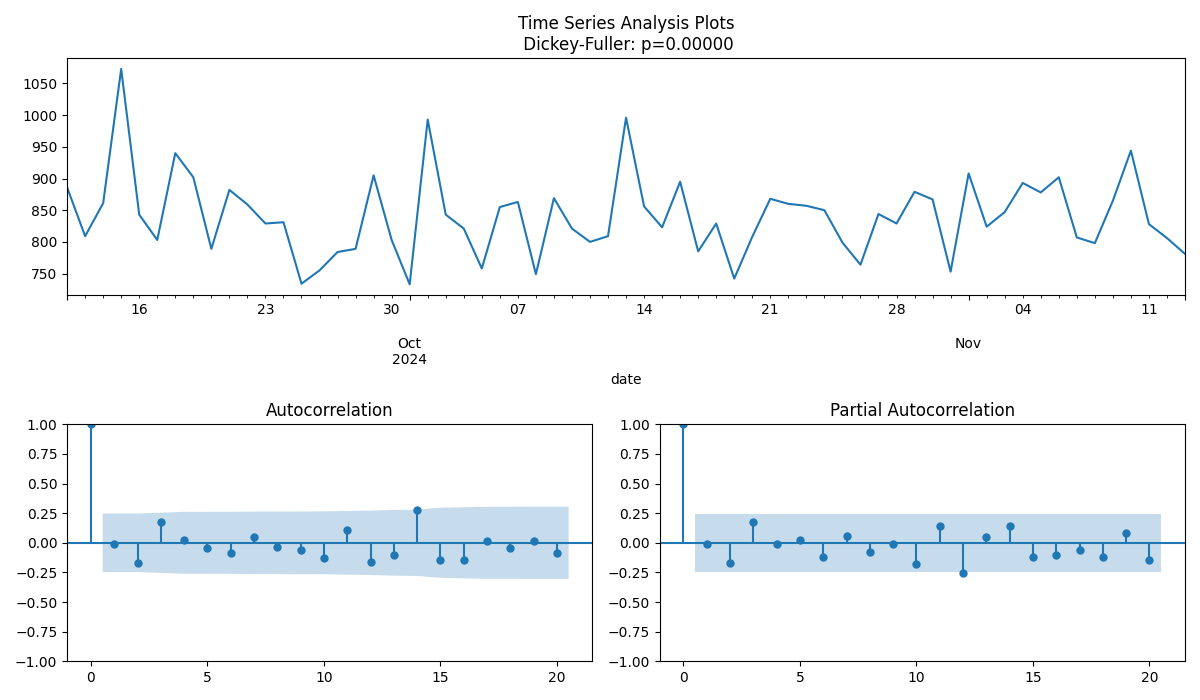
\includegraphics[width=0.5\linewidth]{1a_acf_pacf.png}
    \caption{Time Series Analysis plots}
\end{figure}

\begin{figure}[H]
    \centering
    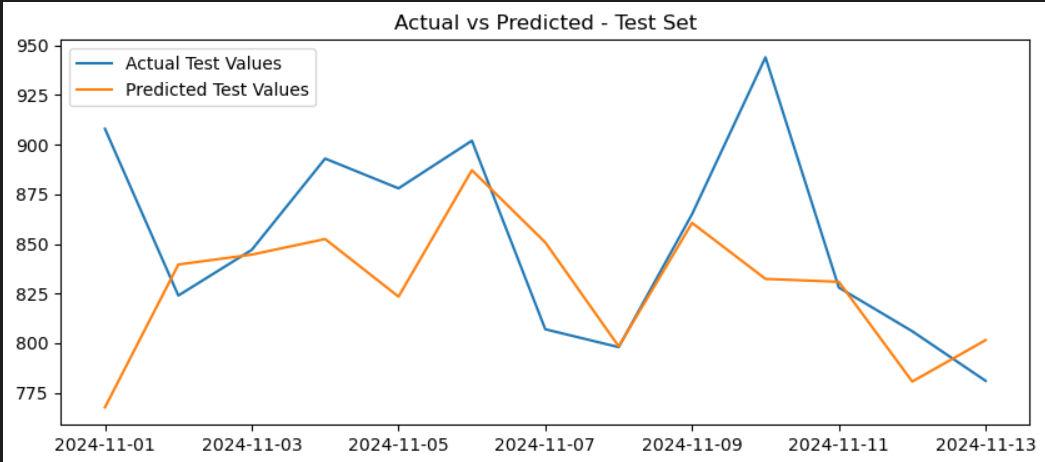
\includegraphics[width=0.5\linewidth]{Screenshot 2024-10-29 004452.png}
    \caption{Test data and forecast}
\end{figure}

\begin{figure}[H]
    \centering
    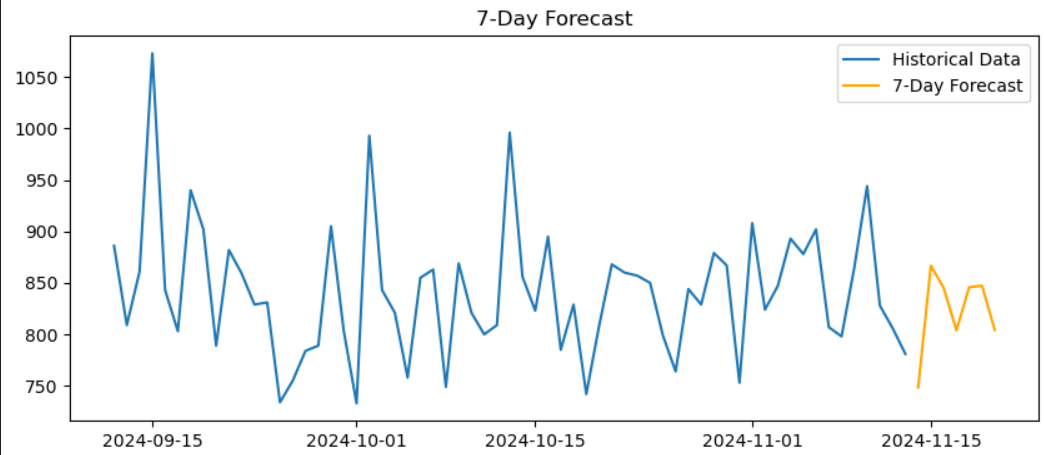
\includegraphics[width=0.5\linewidth]{Screenshot 2024-10-29 004701.png}
    \caption{Forecasted plot}
\end{figure}


\subsection{Forecasting average time spent}

We have forecasted the average time spent using the \textbf{SARIMAX} model.
The parameters \texttt{order=(3, 1, 3)} and \texttt{seasonal\_order=(2, 1, 5, 7)} were used.
We have obtained MAPE: 0.28 and MASE: 0.55. The plots obtained are here:

\begin{figure}[H]
    \centering
    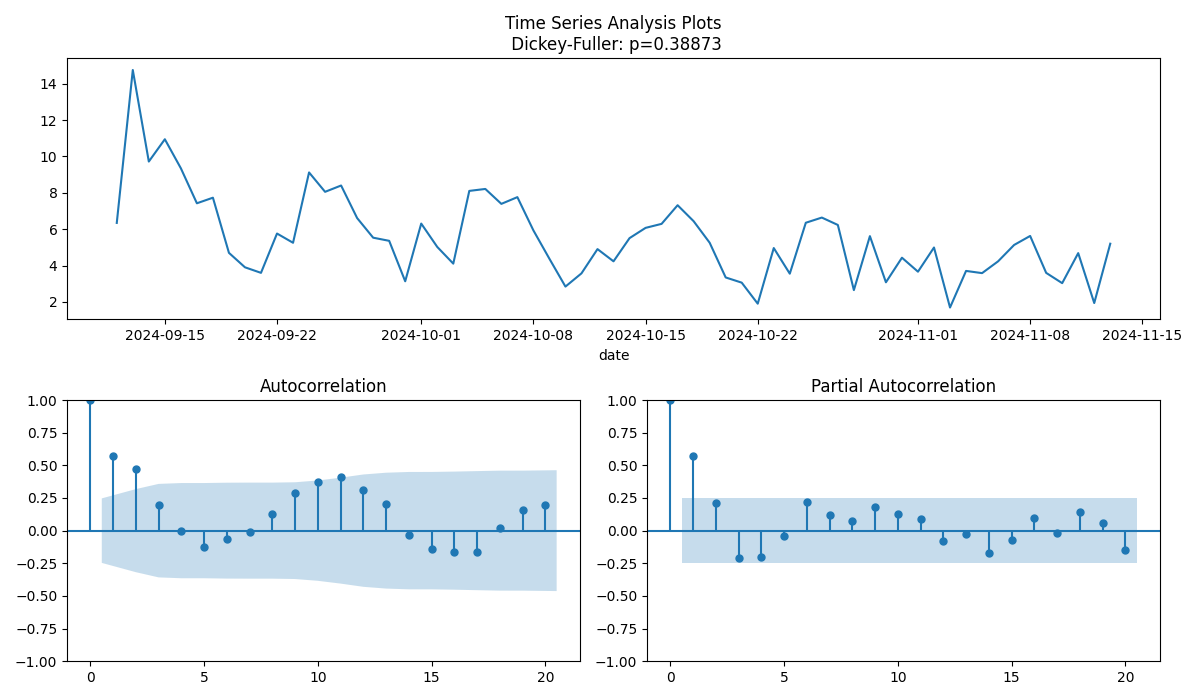
\includegraphics[width=0.5\linewidth]{1b_acf_pacf.png}
    \caption{Time Series Analysis plots}
\end{figure}

\begin{figure}[H]
    \centering
    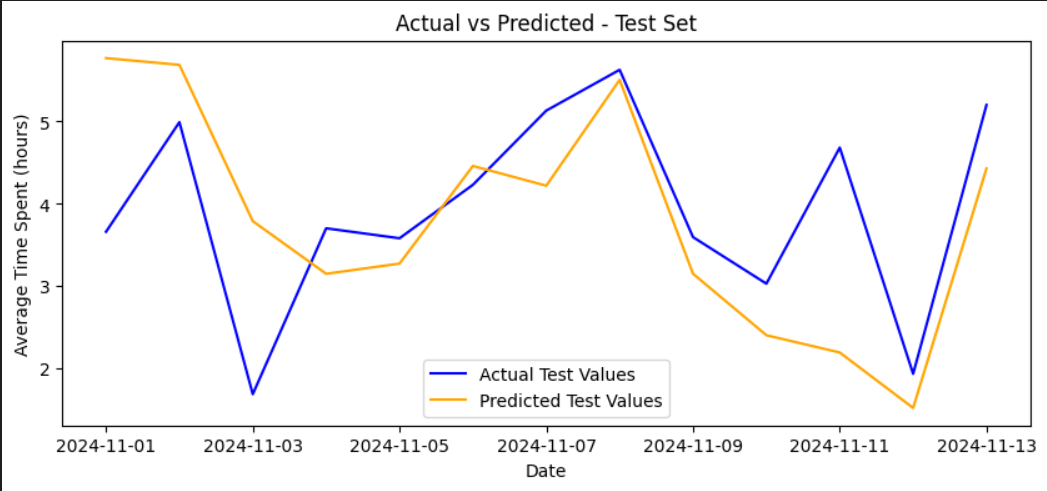
\includegraphics[width=0.5\linewidth]{image.png}
    \caption{Test data and forecast}
\end{figure}

\begin{figure}[H]
    \centering
    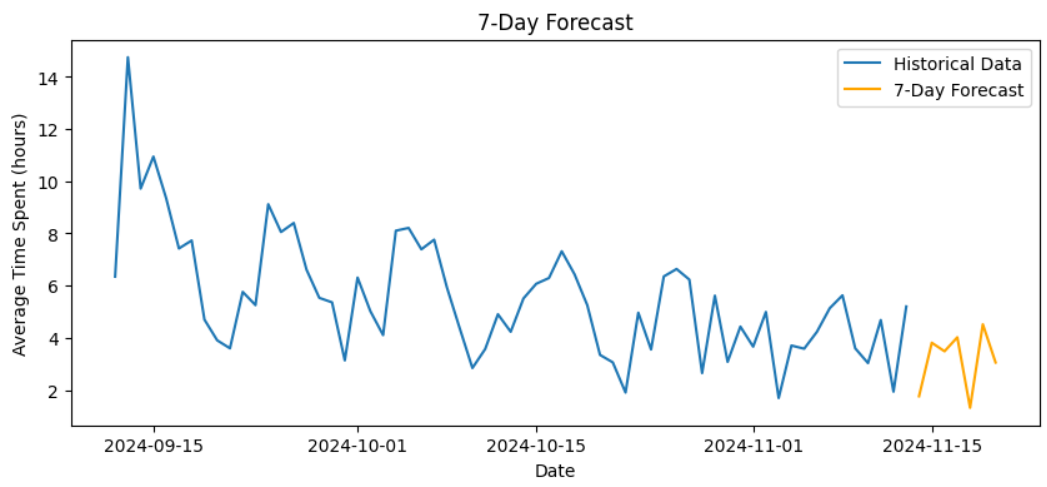
\includegraphics[width=0.5\linewidth]{Screenshot 2024-10-29 004121.png}
    \caption{Forecasted plot}
\end{figure}

\subsection{Smoothing strategies}

We have used two strategies for smoothing of the data:
\begin{itemize}
    \item Moving average smoothing
    \item Exponential smoothing
\end{itemize}
The code can be seen in \texttt{Q1c.ipynb}.

\section{Forecasting on a Real World Dataset}

\subsection{Predicting \texttt{PASSENGERS} \texttt{CARRIED} from 2023 September
to 2024 August}

\subsubsection{Using ARIMA model to forecast the data}

We first cleaned the data by removing unnecessary whitespaces. We also renamed
the months with an index to make it into an iterable format, following which we
applied the \textbf{ARIMA} model to the data to predict future data. Note that we
\textbf{included COVID-19} in the data as it is a prominent feature that
shouldn't be ignored.

We have tried the ARIMA plots for various parameters until we settled for
\texttt{ARIMA(order=(10, 1, 10))}.

The \textbf{ACF} and the \textbf{PACF} plots are

\begin{figure}[H]
  \centering
  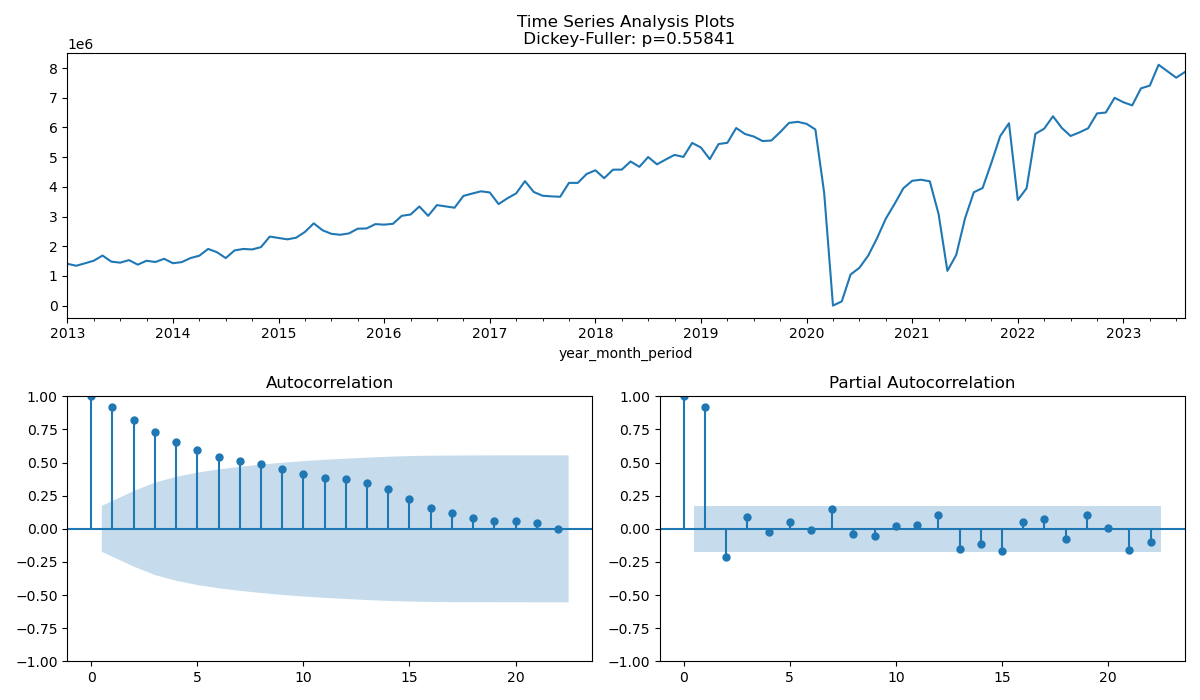
\includegraphics[width=0.7\textwidth]{TSPlot-2-1a.png}
  \caption{Time Series Analysis Plots}
\end{figure}

and the ARIMA model predictions are

\begin{figure}[H]
  \centering
  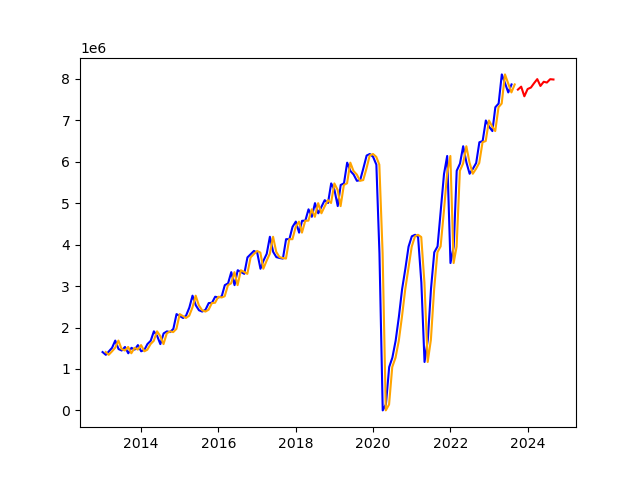
\includegraphics[width=0.7\textwidth]{ARIMA.png}
  \caption{ARIMA applied (The red is the predicted part)}
\end{figure}

The \texttt{submission.csv} file in Kaggle gives a score of 2.84.

\subsubsection{Using an LLM for prediction}

Input prompt to LLM (Google AI Studio):

\begin{verbatim}
Given the following monthly airline passenger data, predict and display
the values for next 12 months (2023 SEP to 2024 AUG) for Passengers Carried,
you need not show any code or your though process, just the final predicted
values must be displayed, there's a season of 4 months: Airline A007, Year
2023, Month JAN, Passengers Carried: 6847384.0. Airline A007, Year 2023, Month
FEB, Passengers Carried: 6741948.0. Airline A007, Year 2023, Month MAR,
Passengers Carried: 7317288.0. Airline A007, Year 2023, Month APR, Passengers
Carried: 7406440.0. Airline A007, Year 2023, M...complete the prompt by
extracting the data from the attached CSV, after removing the covid null
values

-- The CSV file contents --
\end{verbatim}

\noindent The output of the LLM (in Markdown):

\begin{verbatim}
* **2023 SEP:** 79,02,627
* **2023 OCT:** 79,58,513
* **2023 NOV:** 80,12,872
* **2023 DEC:** 80,65,695
* **2024 JAN:** 73,42,625
* **2024 FEB:** 72,37,189
* **2024 MAR:** 78,02,983
* **2024 APR:** 78,92,132
* **2024 MAY:** 85,92,379
* **2024 JUN:** 84,76,054
* **2024 JUL:** 82,57,578
* **2024 AUG:** 84,49,947
\end{verbatim}

\subsubsection{Using Prophet for model fitting}

The Prophet model was used to make the data prediction. The output data graph:
\begin{figure}[H]
  \centering
  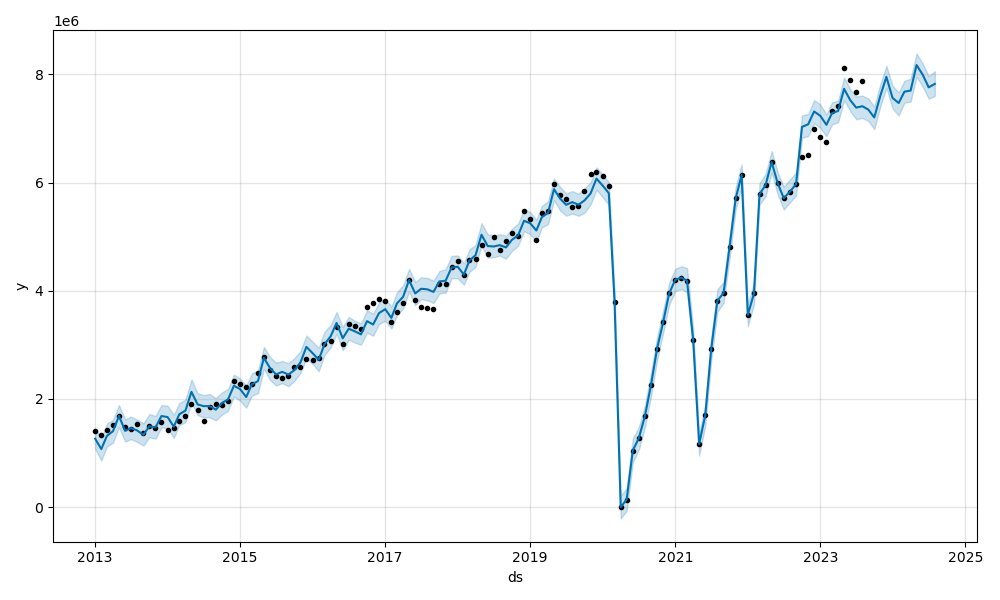
\includegraphics[width=0.8\textwidth]{Prophet.png}
  \caption{Model fitting using Prophet}
\end{figure}
The predicted values are:
\begin{verbatim}
YEAR_MONTH,PASSENGERS CARRIED
2023 SEP,7352169.4825807
2023 OCT,7210166.934052202
2023 NOV,7614914.074459398
2023 DEC,7957471.519386159
2024 JAN,7568591.618646984
2024 FEB,7475801.199378586
2024 MAR,7686314.721362665
2024 APR,7705897.56702898
2024 MAY,8178199.290168875
2024 JUN,7999134.73277676
2024 JUL,7766336.116382452
2024 AUG,7829486.003933291
\end{verbatim}

\subsection{Metrics to evaluate forecasts}

The \textbf{fleet requirement} is constrained by the total number of passengers expected. Hence, there is a greater need for better forecasting during periods of high demand than during periods of low demand. The \textbf{human resources requirement} is constrained by the peak demand. Hence, the forecast for the peak demand must be accurate, i.e., the error must be more sensitive to the peaks.

\subsubsection*{Disadvantages of MAPE}

\begin{itemize}
    \item MAPE calculates the average percentage error across all periods and hence does not differentiate between high and low demand periods.
    \item When the actual values are small, the MAPE will show high sensitivity to the errors. In reality, the errors at low demand are not operationally significant.
\end{itemize}

\subsubsection*{Alternative evaluation metrics}

\begin{itemize}
    \item Weighted Absolute Percentage Error (WAPE) is a better alternative to MAPE. This is because it shows high sensitivity towards errors at high values. This addresses the requirement of better prediction at the peaks.
    \item Root Mean Squared Error (RMSE) is also a good metric because higher deviation during peaks impacts more than MAPE.
\end{itemize}

\subsection{Test to study $\mu$}

To test if $\mu$ is different before and after COVID, we can use the \textbf{t-test} considering the two periods as two samples. In this test, the statistic
\begin{equation*}
    t = \frac{\bar{x} - \mu}{s/\sqrt{n}}
\end{equation*}
is used, where $s$ is the sample standard deviation.

\end{document}
